% !TeX root = ./main.tex
% !TEX program = xelatex

\documentclass[12pt]{article}
\usepackage{graphicx}
\usepackage{fullpage}
\usepackage{enumitem}
\usepackage{amsmath}
\usepackage{tikz}
\usetikzlibrary{arrows}
\usepackage{listings}
\usepackage{algorithm}
\usepackage[noend]{algpseudocode}
\usepackage{multicol}
\usepackage{microtype}
\usepackage{graphicx}
\usepackage[export]{adjustbox}
\usepackage{hyperref}
\hypersetup{
    colorlinks,
    citecolor=black,
    filecolor=black,
    linkcolor=black,
    urlcolor=black
}
\newcommand{\myparagraph}[1]{\paragraph{#1}\mbox{}\\}


%% Language and font encodings
\usepackage[utf8]{inputenc}
\usepackage{xunicode}
\usepackage{xltxtra}
\usepackage{amsfonts, amsmath}
\usepackage[english,greek]{babel}
\usepackage{tcolorbox}

%\usepackage{xgreek}

\setmainfont[Mapping=tex-text]{CMU Serif}
\begin{document}
\sloppy
\begin{titlepage}



\newcommand{\HRule}{\rule{\linewidth}{0.5mm}}
\center

\includegraphics[width=50mm,scale=0.5]{imgs/logo.png}\\[1cm]
\textsc{\LARGE ΕΘΝΙΚΟ ΜΕΤΣΟΒΙΟ ΠΟΛΥΤΕΧΝΕΙΟ}\\[0.05cm] % Name of your university/college
\textsc{\textbf{\Large ΣΧΟΛΗ ΗΛΕΚΤΡΟΛΟΓΩΝ ΜΗΧΑΝΙΚΩΝ \\ \& ΜΗΧΑΝΙΚΩΝ ΥΠΟΛΟΓΙΣΤΩΝ}}\\[1.cm] % Major heading such as course name

\vspace{05mm}
\HRule \\[0.4cm]
{ \huge \bfseries Άσκηση 3 - Προηγμένα Θέματα Αρχιτεκτονικής Υπολογιστών }\\[0.4cm] 
\HRule \\[1.5cm]
 
\center
{\Large Γρηγόριος Θανάσουλας \\ \vspace{1em} gregthanasoulas@gmail.com \\ \vspace{5mm} \Large A.M: 03114131} \\
\vspace{15mm}

{\large \today} % Date, change the \today to a set date if you want to be precise
\vfill

\end{titlepage}
\newpage
\tableofcontents
\newpage

\large{
\setcounter{tocdepth}{3}
\setcounter{secnumdepth}{3}
\section{Σκοπός}
\vspace{3mm}

Η άσκηση αυτή αποσκοπεί στη μελέτη των χαρακτηριστικών των σύγχρονων
superscalar, out-of-order επεξεργαστών και του τρόπου με τον οποίο αυτά
επηρεάζουν την απόδοση του συστήματος, την κατανάλωση ενέργειας καθώς και το
μέγεθος του chip του επεξεργαστή. Για την αξιολόγηση τους γίνεται χρήση του
εργαλείου Sniper Multicore Simulator με τα παρακάτω μετροπρογράμματα (SPEC CPU2006 benchmarks): 

\begin{enumerate}
  \item 403.gcc 
  \item 429.mcf 
  \item 434.zeusmp
  \item 436.cactusADM 
  \item 445.gobmk
  \item 450.soplex
  \item 456.hmmer
  \item 458.sjeng
  \item 459.GemsFDTD
  \item 471.omnetpp
  \item 473.astar
  \item 483.xalancbmk
\end{enumerate}}

\vspace{3mm}

\section{Πειραματική Αξιολόγηση}
\subsection{Ερώτημα i}
Ζητείται να εκτελέσουμε όλα τα benchmarks για κάθε διαφορετικό επεξεργαστή που
προκύπτει από το συνδυασμό των παρακάτω τιμών για τις παραμέτρους dispatch\_width
και window\_size:

\begin{center}
   \vspace{3mm}
   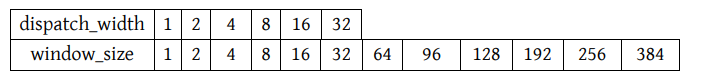
\includegraphics[width=0.9\textwidth]{./imgs/combos.png}
   \vspace{3mm}
\end{center}

\noindent Από τους παραπάνω $6 \times 12  = 72$ δυνατούς συνδυασμούς νόημα έχουν
μόνο εκείνοι για τους οποίους ισχύει $window\_size \geq dispatch\_width$. Αυτό
μπορεί να αιτιολογηθεί θεωρητικά ως εξής: για να γίνει μία εντολή issue πρέπει
να υπάρχει διαθέσιμη θέση στον ROB. Επομένως, είναι χωρίς νόημα να κάνουμε
dispatch παραπάνω εντολές από όσες μπορούν να χωρέσουν στον Reorder Buffer,
γιατί απλά αυτές θα περιμένουν μέχρι να υπάρξει ελεύθερη θέση στον ROB και άρα η
επίδοση δε θα βελτιωθεί καθόλου. Με βάση αυτό αγνοούμε για οικονομία χρόνου στις
προσομοιώσεις τους συνδυασμούς για τους οποίους $window\_size < dispatch\_width$
και εκτελούμε τους υπόλοιπους 57 συνδυασμούς. 

Την παρατήρηση αυτή μπορούμε να επιβεβαιώσουμε και πειραματικά. Στα παρακάτω
διαγράμματα απεικονίζεται η μετρική Instructions Per Cycle για τα
μετροπρογράμματα gcc και sjeng για όλους τους δυνατούς συνδυασμούς. Παρατηρούμε
πως για κάθεμία από τις καμπύλες των διαγραμμάτων (που ανατιστοιχεί σε ορισμένο
dispatch width), η απόδοση (μετρική IPC) για τις τιμές windows\_size που είναι
μκρότερες από το dispatch width είναι πάντα χαμηλότερη από την επίδοση στους
υπόλοιπους συνδυασμούς.

\vspace{3mm}
   \begin{minipage}{\textwidth}
      \begin{center}
         \fbox{\textlatin{\textbf{\textit{403-gcc}}}}\\
         \vspace{3mm}
         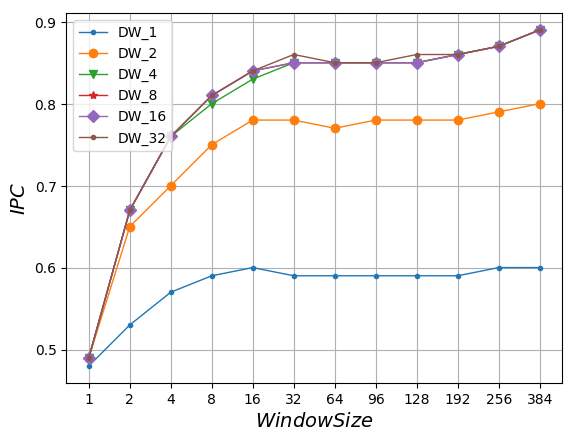
\includegraphics[width=0.7\textwidth, frame]{./graphs/ipc/gcc.png}
         \vspace{6mm}
      \end{center}
   \end{minipage}

   \begin{minipage}{\textwidth}
      \begin{center}
         \fbox{\textlatin{\textbf{\textit{458-sjeng}}}}\\
         \vspace{3mm}
         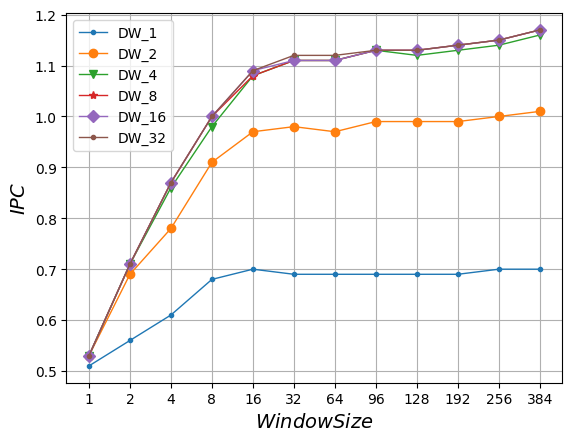
\includegraphics[width=0.7\textwidth, frame]{./graphs/ipc/sjeng.png}
         \vspace{6mm}
      \end{center}
   \end{minipage}

\newpage
\subsection{Ερώτημα ii}

\begin{tcolorbox}
Για την μελέτη των χαρακτηριστικών εκτελέσαμε τα 12 παραπάνω benchmarks για τους
συνδυασμούς χαρακτηριστικών επεξεργαστή που αναφέρθηκαν στο προηγούμενο ερώτημα.
Ωστόσο, πρέπει σε αυτό το σημείο να σημειώσουμε ότι ορισμένα από τα benchmarks
εμφάνιζαν errors κατά την εκτέλεση με αποτέλεσμα η προσομοίωση να εκτελείται για
μικρό αριθμό εντολών, γεγονός που σημαίνει ότι δεν είναι αξιόπιστη η "εικόνα"
της προσομοίωσης αυτής.
Λαμβάνοντας υπ' όψιν βάσει της εκφώνησης της εργαστηριακής άσκησης ότι το κάθε
pinball περιέχει περίπου 1 billion εντολές, και βάσει των αποτελεσμάτων στα
αρχεία sim.out βρέθηκε για το κάθε benchmark ότι εκτελούνται τα παρακάτω ποσοστά
εντολών: 


\begin{center}
   \vspace{3mm}
   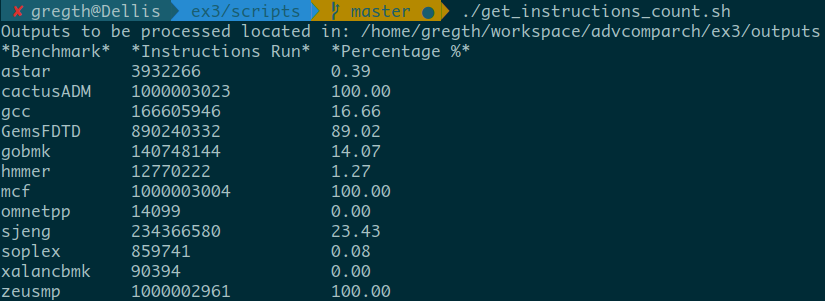
\includegraphics[width= \textwidth]{./imgs/count.png}
   \vspace{2mm}
\end{center}

Από τα benchmarks αυτά, και βάσει τον διευκρινήσεων που δόθηκαν θα κρατήσουμε 
τις προσμοποιώσεις οπου έχει εκτελεστεί παραπάνω από το 10 \% του pinball.
Συνεπώς, δεν έχει νόημα να μελετήσουμε 5 από τα 12 benchmarks,
και συγκεκριμένα τα astar, hmmer, soplex, xalancbmk, omnetpp.

\end{tcolorbox}

\noindent \\Ακολουθούν τα διαγράμματα και ο σχολιασμός τους:

\vspace{3mm}
   \begin{minipage}{\textwidth}
      \begin{center}
         \fbox{\textlatin{\textbf{\textit{403-gcc}}}}\\
         \vspace{3mm}
         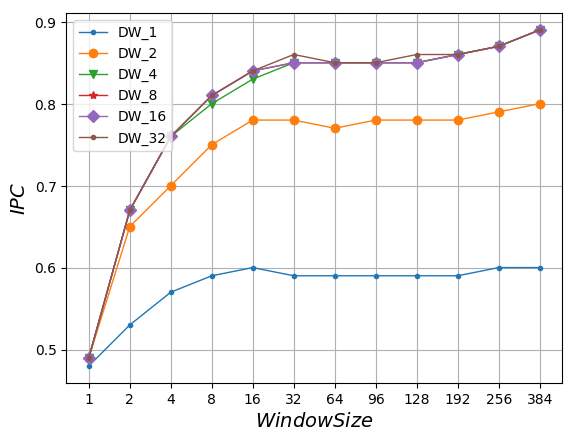
\includegraphics[width=0.7\textwidth, frame]{./graphs/ipc/gcc.png}
         \vspace{6mm}
      \end{center}
   \end{minipage}

   \begin{minipage}{\textwidth}
      \begin{center}
         \fbox{\textlatin{\textbf{\textit{429-mcf}}}}\\
         \vspace{3mm}
         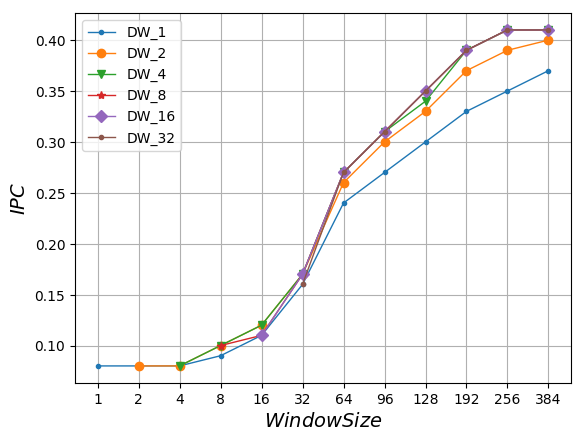
\includegraphics[width=0.7\textwidth, frame]{./graphs/ipc/mcf.png}
         \vspace{6mm}
      \end{center}
   \end{minipage}

   \begin{minipage}{\textwidth}
      \begin{center}
         \fbox{\textlatin{\textbf{\textit{434-zeusmp}}}}\\
         \vspace{3mm}
         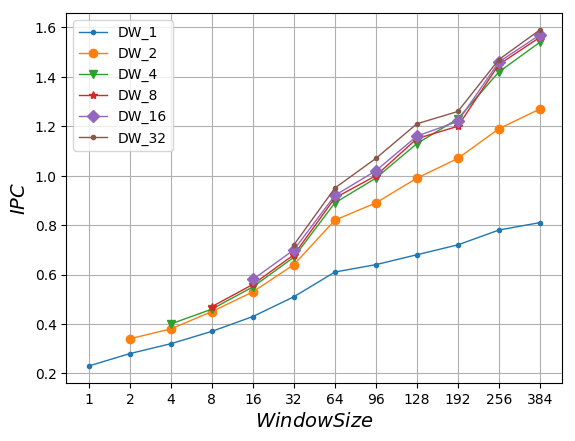
\includegraphics[width=0.7\textwidth, frame]{./graphs/ipc/zeusmp.png}
         \vspace{6mm}
      \end{center}
   \end{minipage}

   \begin{minipage}{\textwidth}
      \begin{center}
         \fbox{\textlatin{\textbf{\textit{436-cactusADM}}}}\\
         \vspace{3mm}
         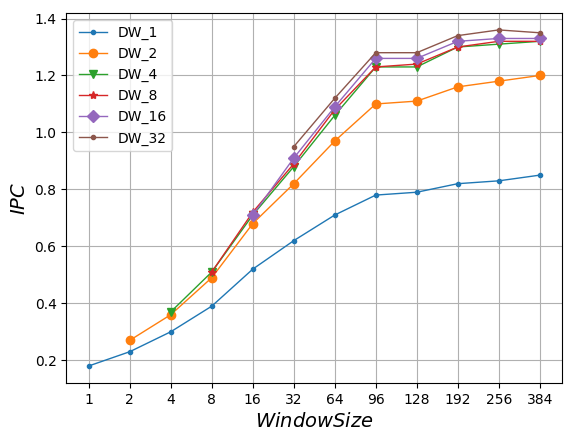
\includegraphics[width=0.7\textwidth, frame]{./graphs/ipc/cactusADM.png}
         \vspace{6mm}
      \end{center}
   \end{minipage}

   \begin{minipage}{\textwidth}
      \begin{center}
         \fbox{\textlatin{\textbf{\textit{445-gobmk}}}}\\
         \vspace{3mm}
         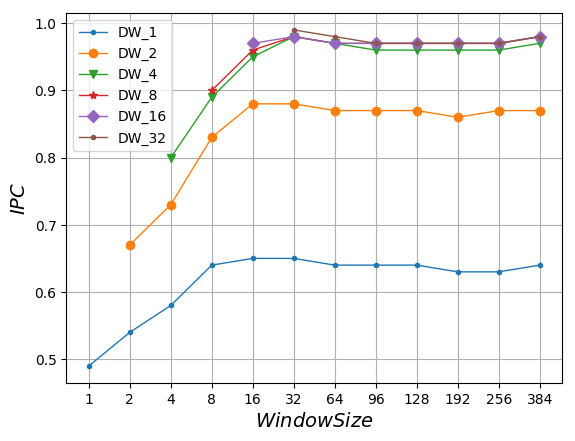
\includegraphics[width=0.7\textwidth, frame]{./graphs/ipc/gobmk.png}
         \vspace{6mm}
      \end{center}
   \end{minipage}

   \begin{minipage}{\textwidth}
      \begin{center}
         \fbox{\textlatin{\textbf{\textit{458-sjeng}}}}\\
         \vspace{3mm}
         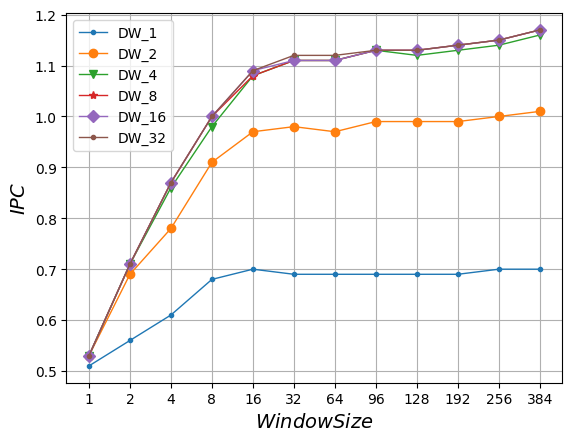
\includegraphics[width=0.7\textwidth, frame]{./graphs/ipc/sjeng.png}
         \vspace{6mm}
      \end{center}
   \end{minipage}

   \begin{minipage}{\textwidth}
      \begin{center}
         \fbox{\textlatin{\textbf{\textit{459-GemsFDTD}}}}\\
         \vspace{3mm}
         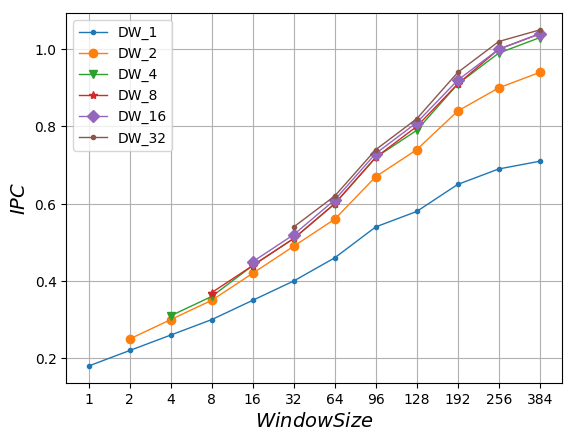
\includegraphics[width=0.7\textwidth, frame]{./graphs/ipc/GemsFDTD.png}
         \vspace{6mm}
      \end{center}
   \end{minipage}


   \paragraph{Συμπεράσματα - Σχόλια}
   Από τις παραπάνω γραφικές του IPC συναρτήσει των dispatch width και window
   size μπορούμε εύκολα να συμπεράνουμε ότι η αύξηση του dispatch width από 1 σε
   2 και από 2 σε 4 εντολές επιφέρει σημαντική βελτίωση της επίδοσης. Ωστόσο,
   περαιτέρω αύξηση σε του dispatch width σε 8, 16 ή και 32 εντολές δεν επιφέρει
   σημαντική αλλαγή στην επίδοση (οι γραφικές για τις τιμές αυτές είναι ως επί
   το πλείστον επικαλυπτόμενες) και άρα δεν έχει νόημα.

   Αυτό μπορεί να ερμηνευθεί λόγω των περιορισμών του ILP (Instruction Level
   Parallelism) του κώδικα που εκτελείται. Δηλαδή, είναι δύσκολο να υπαρξουν και
   να γίνουν issue μεγάλες πλειάδες εντολών (κάθε πλειάδα πάνω από 4 εντολές)
   που να είναι ανεξάρτητες μεταξύ τους ώστε να μπορούν να γίνουν process
   παράλληλα και να επιτύχουμε με ικανοποιητικό ipc. 


   Όσον αφορά το window size, δηλαδή το μέγεθος του Reorder Buffer, βλέπουμε πως
   καθώς αυξάνεται, αυξάνεται συνήθως και το ipc. Αναλυτικότερα, υπάρχουν
   benchmarks (gemsFDTD, cactusADM, zeusmp, mcf)  που αυτή η αύξηση συνεχίζεται
   διαρκώς καθώς αυξάνεται το μέγεθος του ROB, λαμβάνοντας μέγιστη τιμή για το
   μεγαλύτερο window size = 384 και άλλα benchmarks (sjeng, gobmk, gcc) για τα
   οποία η αύξηση είναι σημαντική μέχρι ενός ορίου windows size = 32 περίπου,
   και από το σημείο αυτό και πέρα η αύξηση του ipc δεν είναι τόσο σημαντική.
   Αξίζει επίσης να σημειώσουμε ότι στα benchmarks zeusmp, cactusADM, sjeng,
   GemsFDTD το IPC καταφέρνει να ξεπεράσει τη μονάδα για dispatch width = 4 και
   αρκούντως μεγάλο window size.

   Βάσει των παραπάνω, για την κατασκευή θα επιλέγαμε πιθανόττα dispatch width =
   4 και ένα αρκετά μεγάλο window size, το οποίο θα μας υπαγόρευαν άλλοι
   περιορισμοί, όπως η ενέργεια και το κόστος.
\subsection{Ερώτημα iii}
   Ακολουθούν διαγράμματα για το μέγεθος του επεξεργαστή και κατανάλωση ενέργειας.    
   \\
   \begin{minipage}{\textwidth}
      \begin{center}
         \fbox{\textlatin{\textbf{\textit{Chip Area}}}}\\
         \vspace{3mm}
         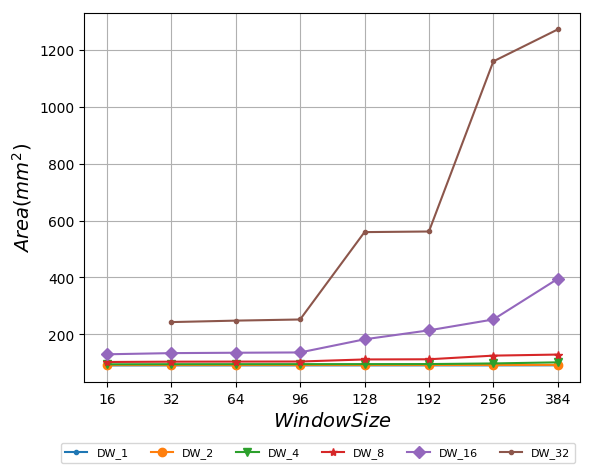
\includegraphics[width=0.7\textwidth]{./graphs/area/area.png}
         \vspace{6mm}
      \end{center}
   \end{minipage}

   \begin{minipage}{\textwidth}
      \begin{center}
         \fbox{\textlatin{\textbf{\textit{403-gcc}}}}\\
         \vspace{3mm}
         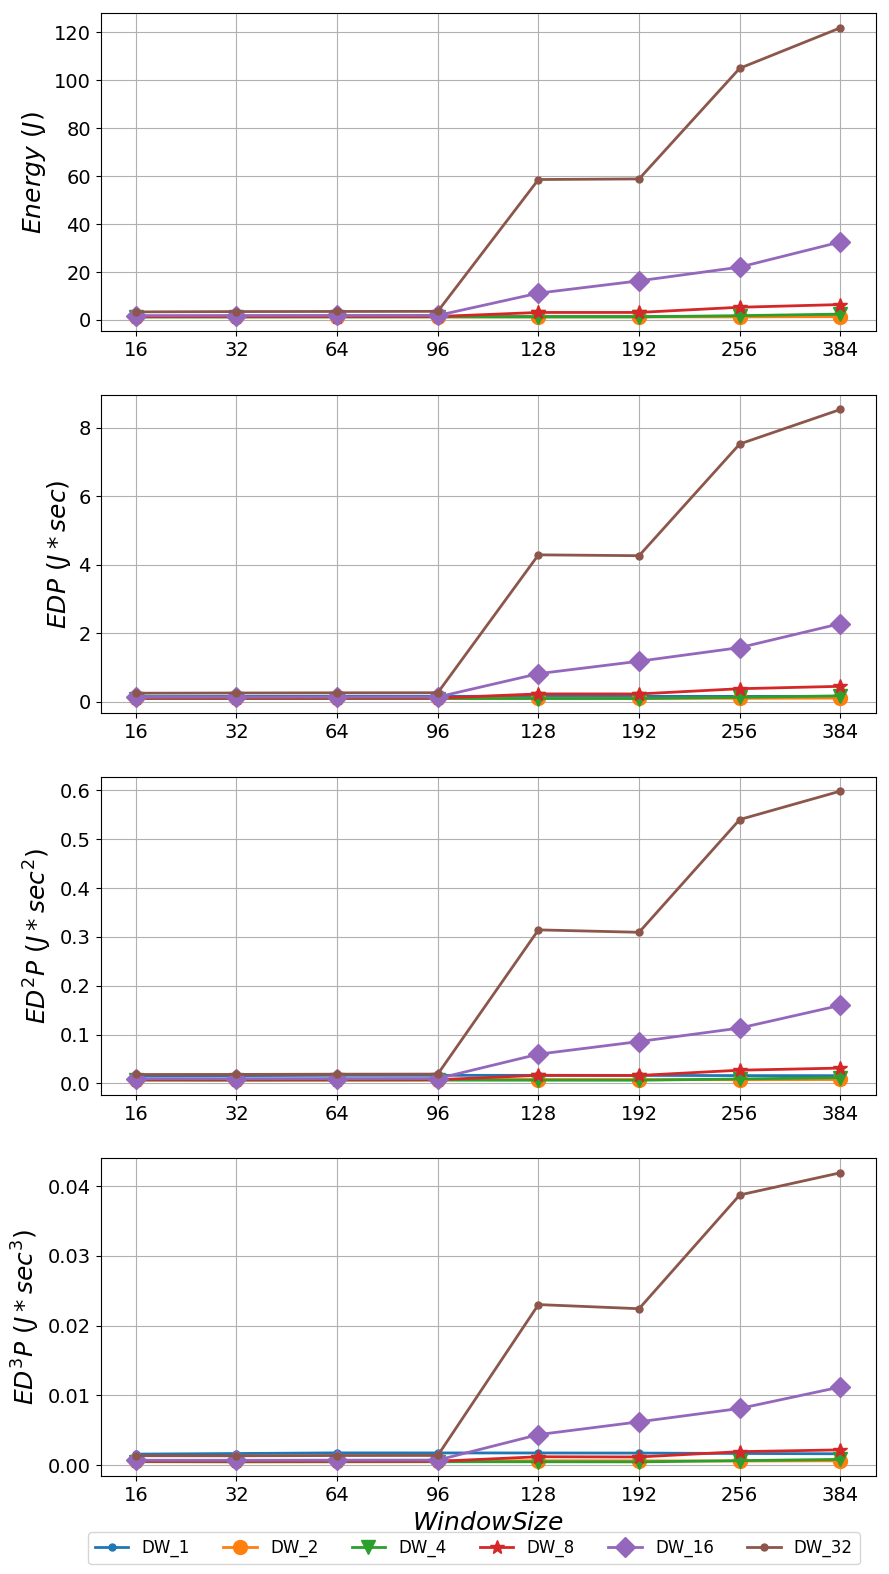
\includegraphics[width=0.6\textwidth]{./graphs/edp/gcc.png}
         \vspace{6mm}
      \end{center}
   \end{minipage}

   \begin{minipage}{\textwidth}
      \begin{center}
         \fbox{\textlatin{\textbf{\textit{429-mcf}}}}\\
         \vspace{3mm}
         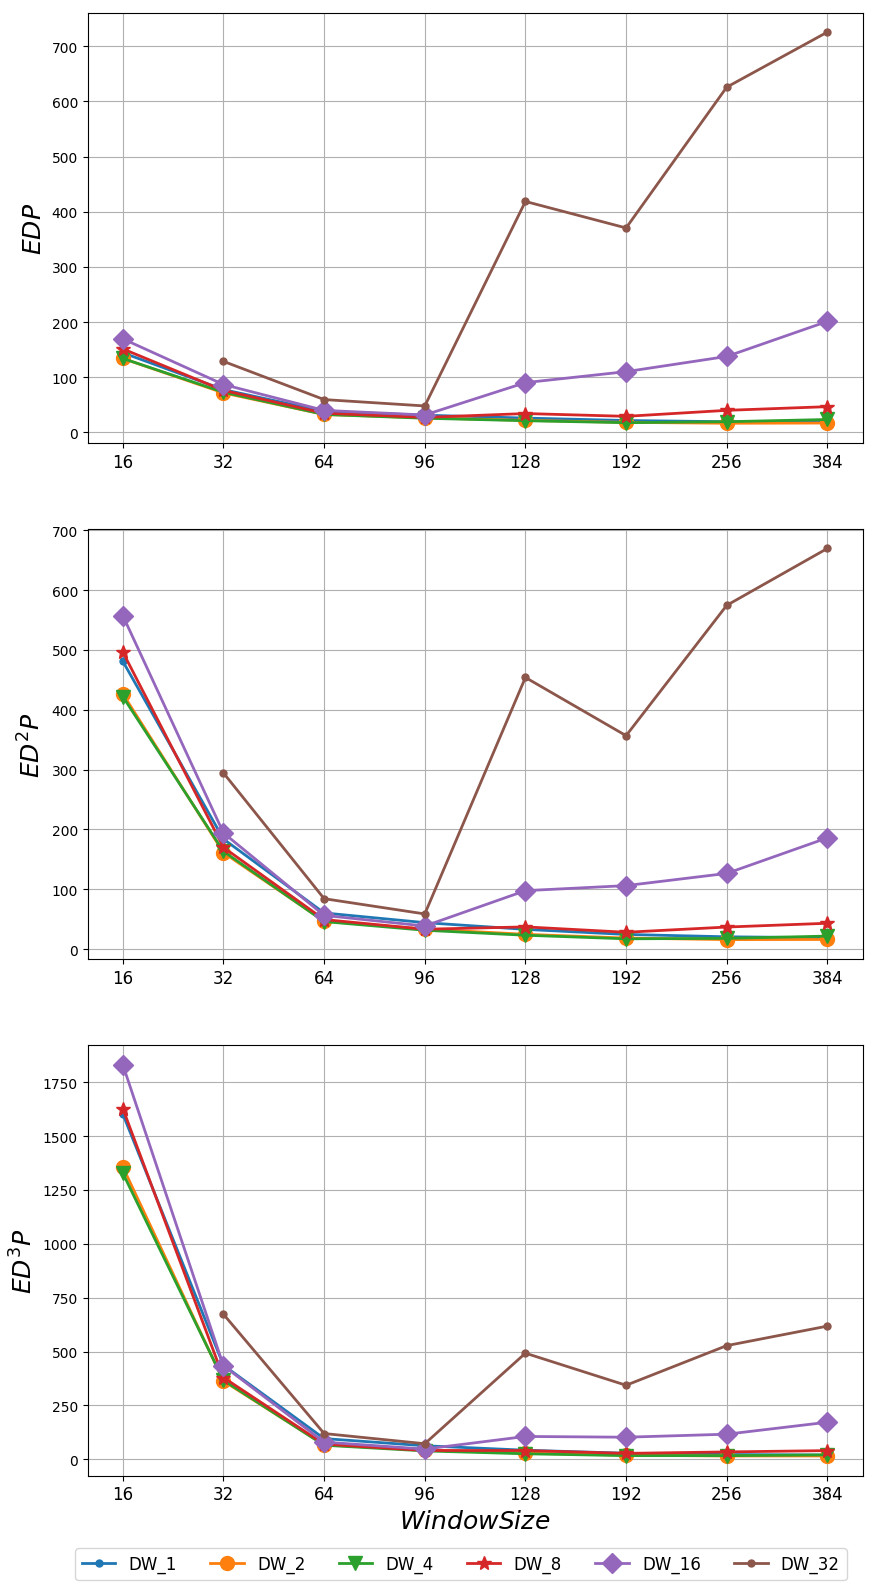
\includegraphics[width=0.7\textwidth]{./graphs/edp/mcf.png}
         \vspace{6mm}
      \end{center}
   \end{minipage}

   \begin{minipage}{\textwidth}
      \begin{center}
         \fbox{\textlatin{\textbf{\textit{434-zeusmp}}}}\\
         \vspace{3mm}
         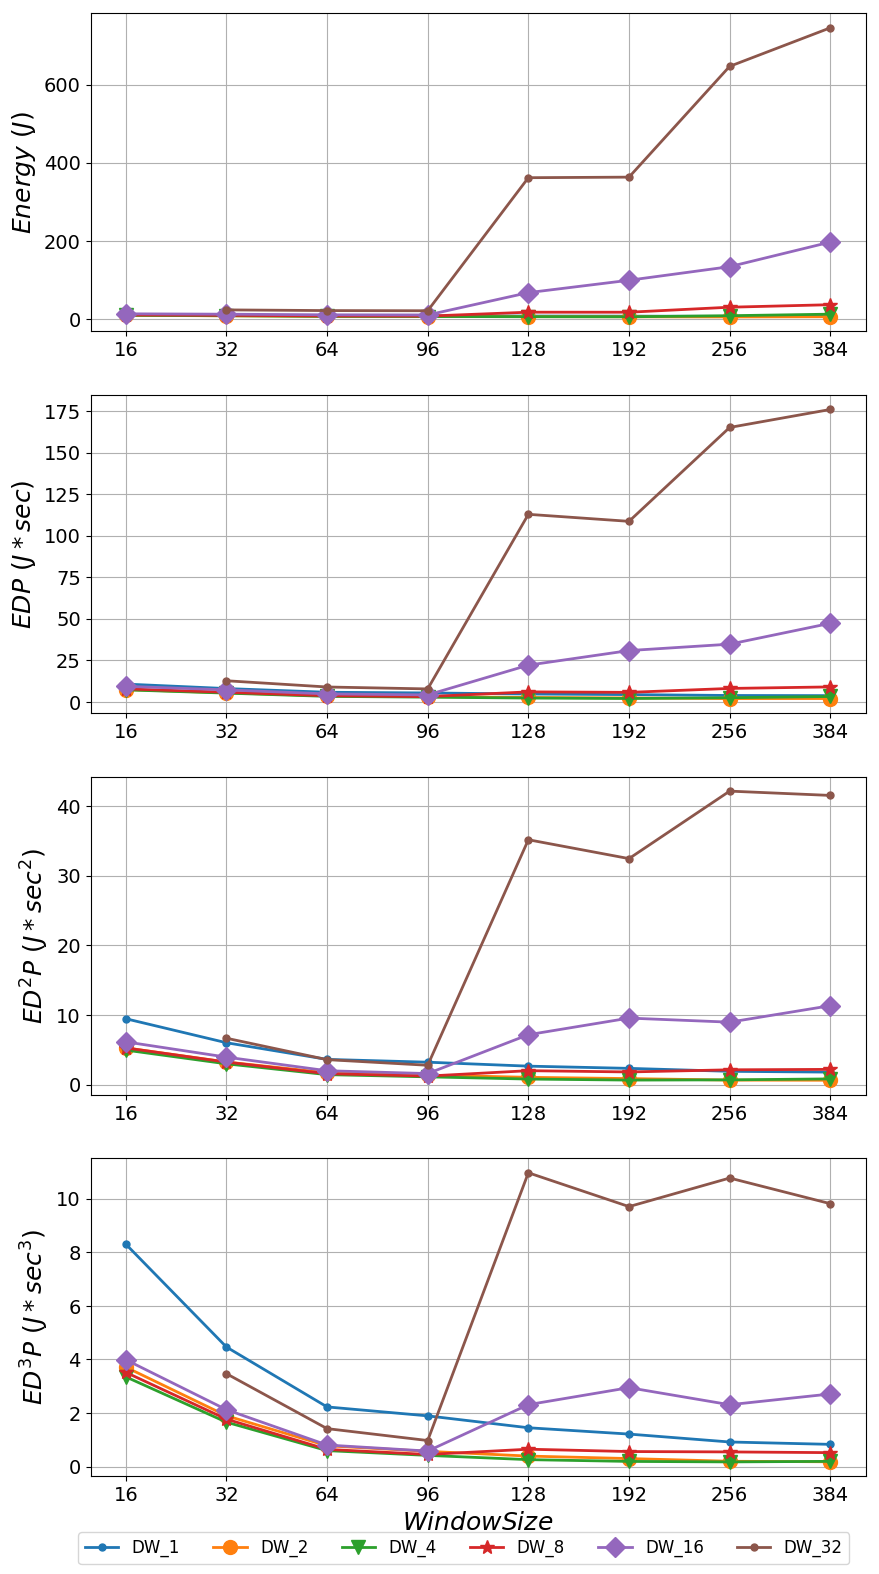
\includegraphics[width=0.7\textwidth]{./graphs/edp/zeusmp.png}
         \vspace{6mm}
      \end{center}
   \end{minipage}

   \begin{minipage}{\textwidth}
      \begin{center}
         \fbox{\textlatin{\textbf{\textit{436-cactusADM}}}}\\
         \vspace{3mm}
         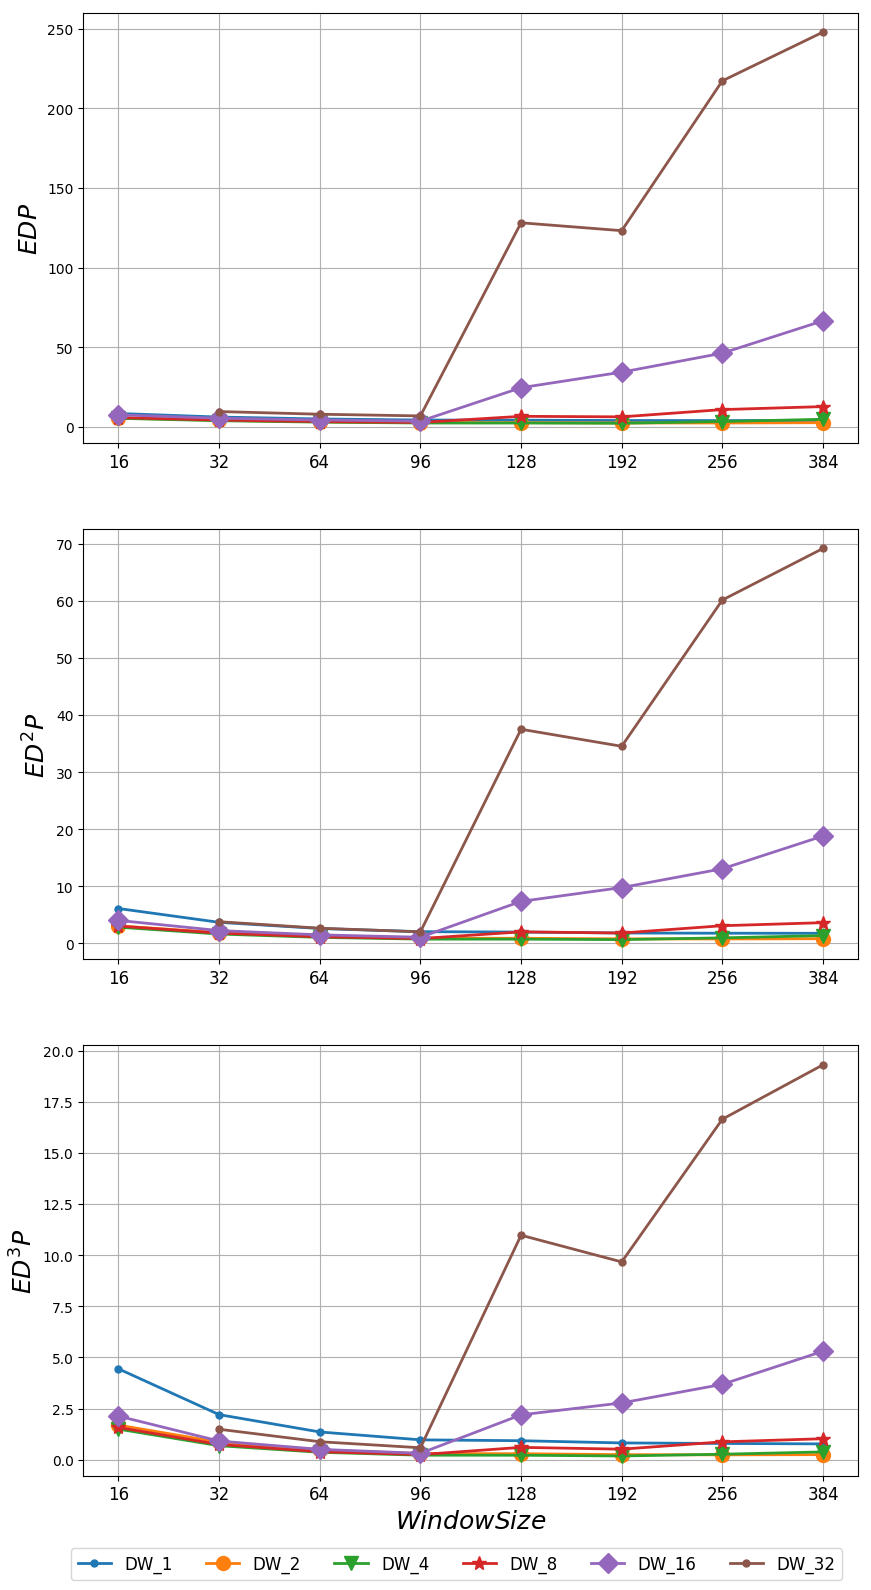
\includegraphics[width=0.7\textwidth]{./graphs/edp/cactusADM.png}
         \vspace{6mm}
      \end{center}
   \end{minipage}

   \begin{minipage}{\textwidth}
      \begin{center}
         \fbox{\textlatin{\textbf{\textit{445-gobmk}}}}\\
         \vspace{3mm}
         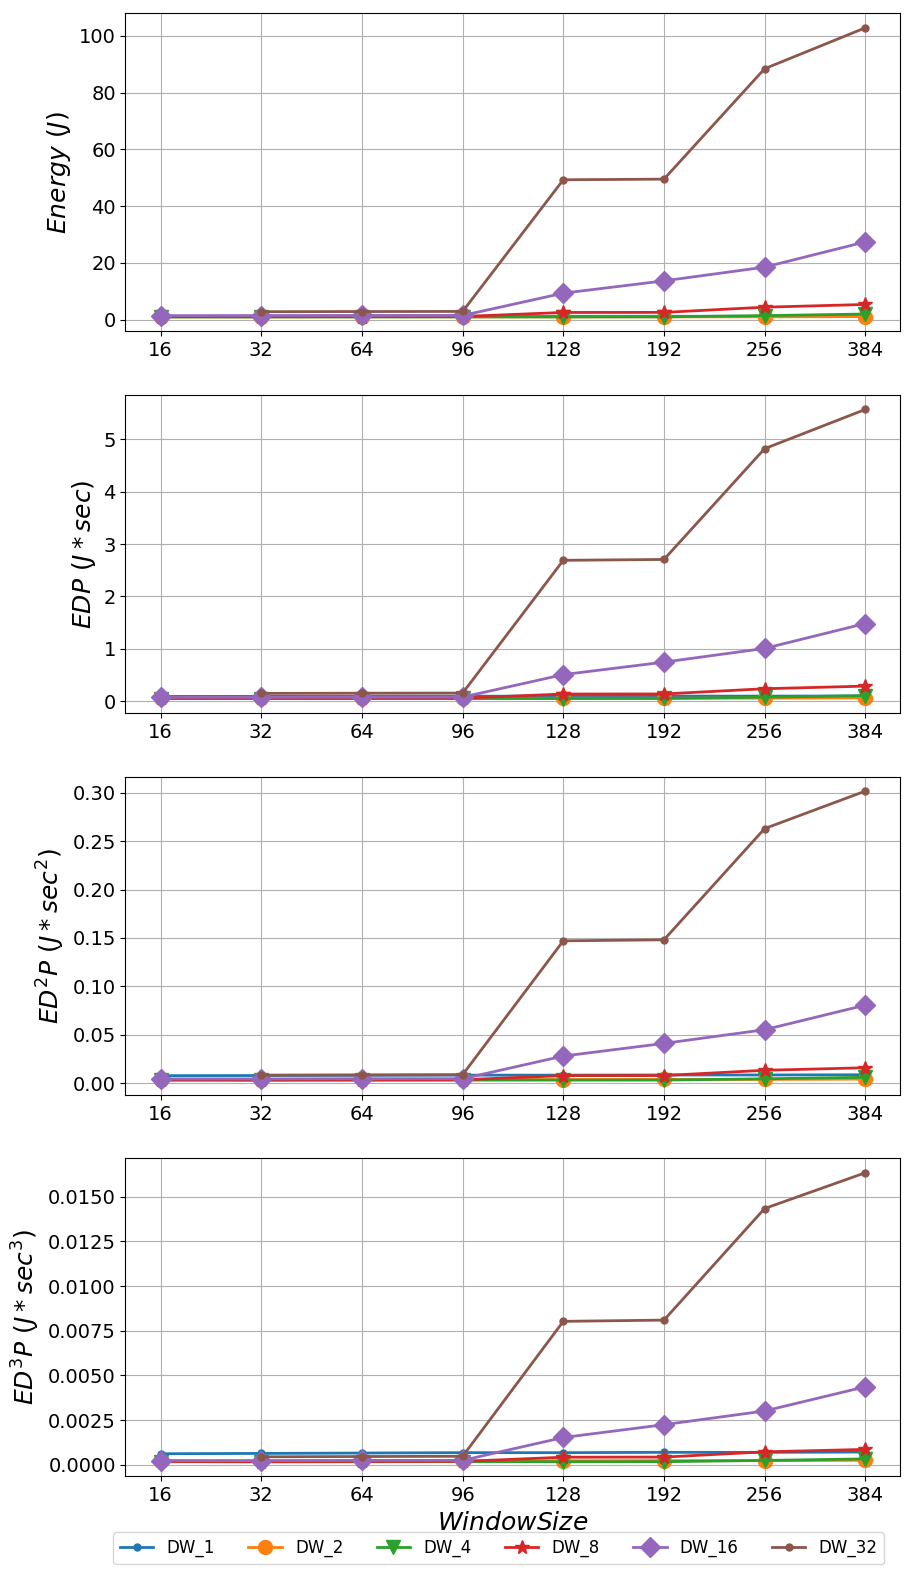
\includegraphics[width=0.7\textwidth]{./graphs/edp/gobmk.png}
         \vspace{6mm}
      \end{center}
   \end{minipage}

   \begin{minipage}{\textwidth}
      \begin{center}
         \fbox{\textlatin{\textbf{\textit{458-sjeng}}}}\\
         \vspace{3mm}
         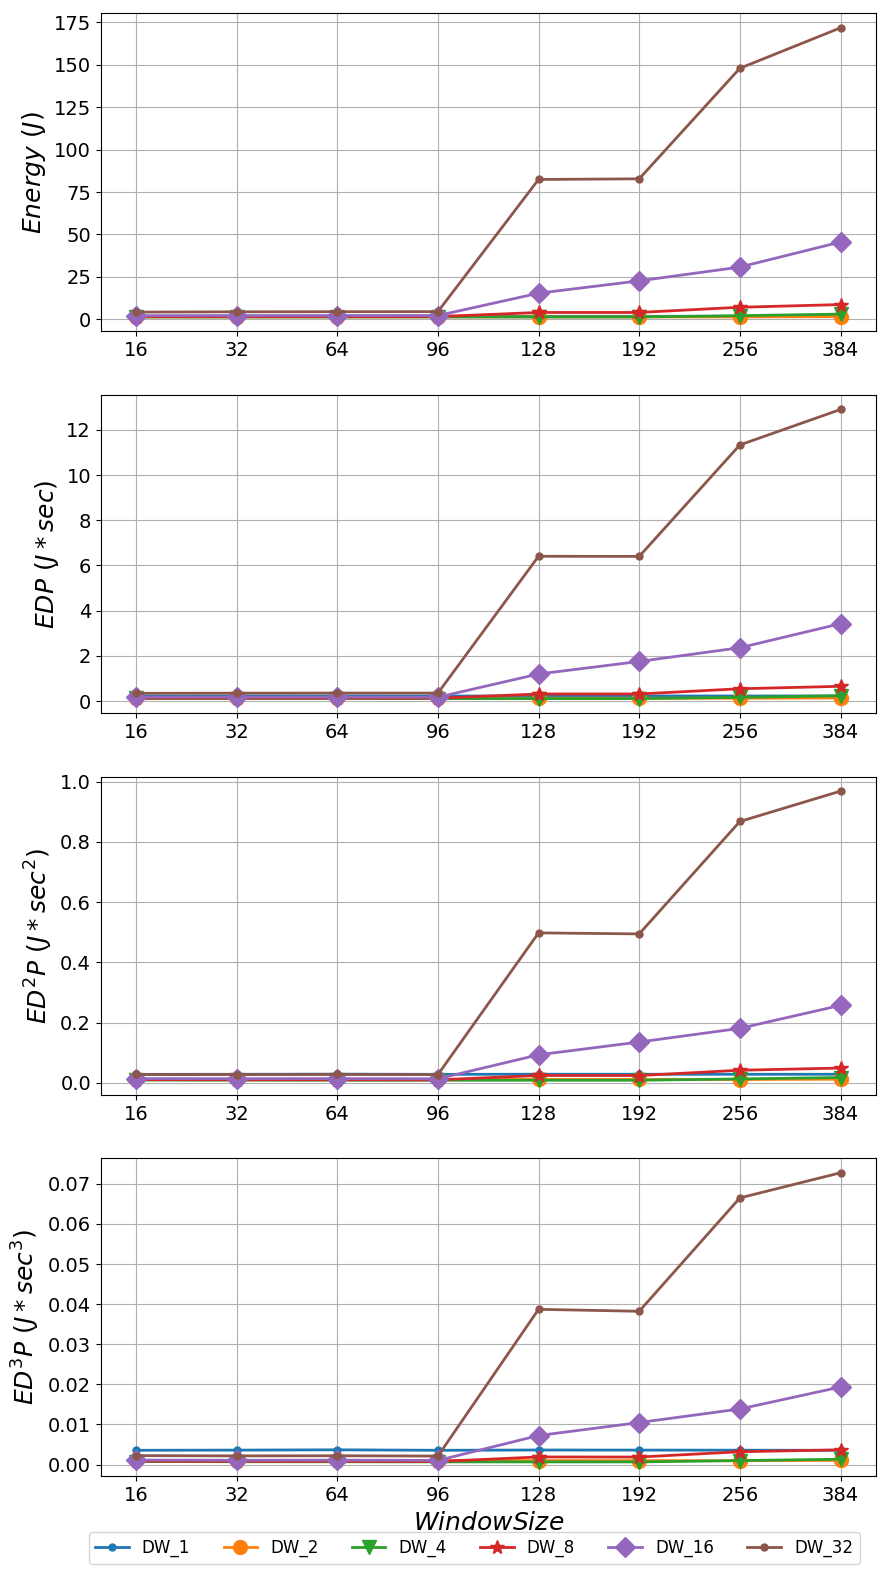
\includegraphics[width=0.7\textwidth]{./graphs/edp/sjeng.png}
         \vspace{6mm}
      \end{center}
   \end{minipage}

   \begin{minipage}{\textwidth}
      \begin{center}
         \fbox{\textlatin{\textbf{\textit{459-GemsFDTD}}}}\\
         \vspace{3mm}
         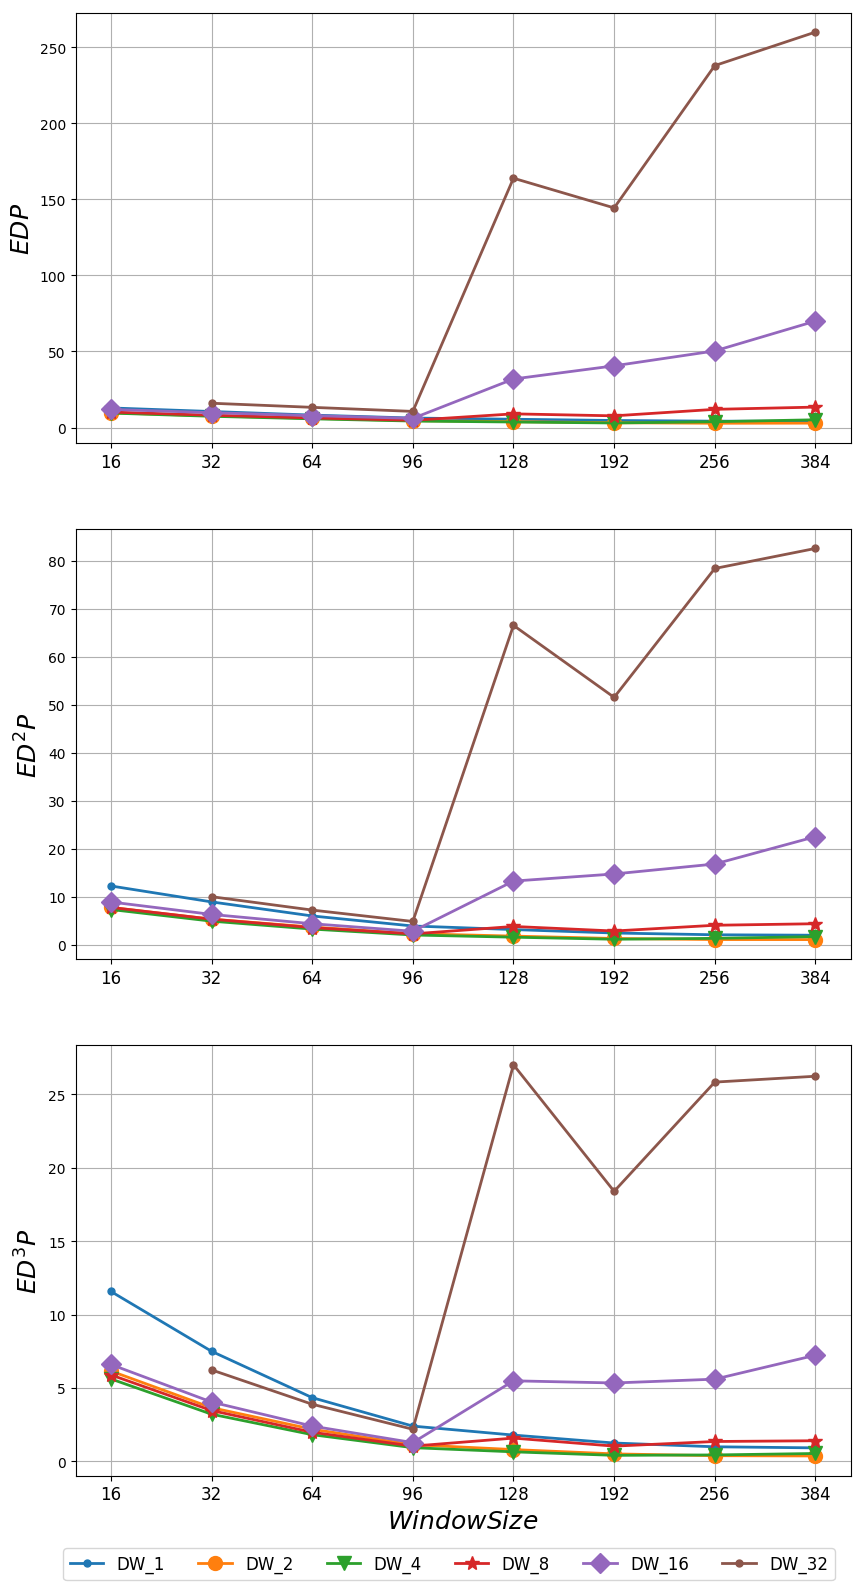
\includegraphics[width=0.7\textwidth]{./graphs/edp/GemsFDTD.png}
         \vspace{6mm}
      \end{center}
   \end{minipage}



   \paragraph{Συμπεράσματα - Σχόλια}
   Αναφορικά με το μέγεθος του chip, παρατηρούμε πως δεν υπάρχει σημαντική
   διαφοροποίηση για επεξεργαστές με dispatch width 1, 2, 4 ή 8 εντολών.
   Μάλιστα, για τις τιμές αυτές του dispatch width το μέγεθος είναι περί τα 100
   με 150 $mm^2$ και δεν μεταβάλλεται σημαντικά καθώς το window size αυξάνει.
   Ωστόσο, για dispatch width 16 και 32 το μέγεθος αυξάνει δραματικά $mm^2$ και
   επηρεάζεται από το window size. Μάλιστα, για dispatch width 32 και window
   size 384 το chip αποκτά το αρκετά μεγάλο μέγεθος $1300 mm^2$.

   Ως προς την ενέργεια που καταναλώνεται, παρατηρούμε ότι σε όλα τα benchmarks
   οι επιμέρους γραφικές για dispatch width 1, 2, 4 και 8 είναι παραπλήσιες, και
   άρα και η ενέργεια που καταναλώνεται είναι περίπου ίδια για ίδιο window size
   και dispatch width  1, 2, 4 ή 8. Παρατηρούμε επίσης πως σε ορισμένα
   benchmarks (mcf, zeus, cactusADM, GemsFDTD) για τις παραπάνω τιμές dispatch
   width και μικρές τιμές window size = 16 ή 32 η ενέργεια είναι πιο μεγάλη σε
   σχέση με λίγο μεγαλύτερο window size. Η ελάχιστη ενέργεια στις περιπτώσεις
   αυτές δείχνει να είναι για window size 128 ή 256. Ωστόσο και για μεγαλύτερα window size δεν υπάρχει σοβαρή επίπτωση.
  
   Η επιλογή dispatch width 16 και 32 αυξάνει δραστικά την ενέργεια που
   καταναλώνεται και μάλιστα στην περίπτωση αυτή αυξάνει σημαντικά καθώς
   αυξάνεται το window size. 
   
   Με βάση την ανάλυση αυτή αλλά και λεμβάνοντας υπόψιν την ανάλυση για την
   επίδοση στα προηγούμενα ερωτήματα, θα επέλεγα dispatch width = 4 και dispatch
   width (δεδομένου ότι η πράσινη καμπύλη είναι φθίνουσα ή σταθερή καθώς αυξάνει
   το window size) τουλάχιστον 256.
\subsection{Ερώτημα iv}
   \begin{minipage}{\textwidth}
      \begin{center}
         \fbox{\textlatin{\textbf{\textit{Kaby Lake Microarchitecture}}}}\\
         \vspace{3mm}
         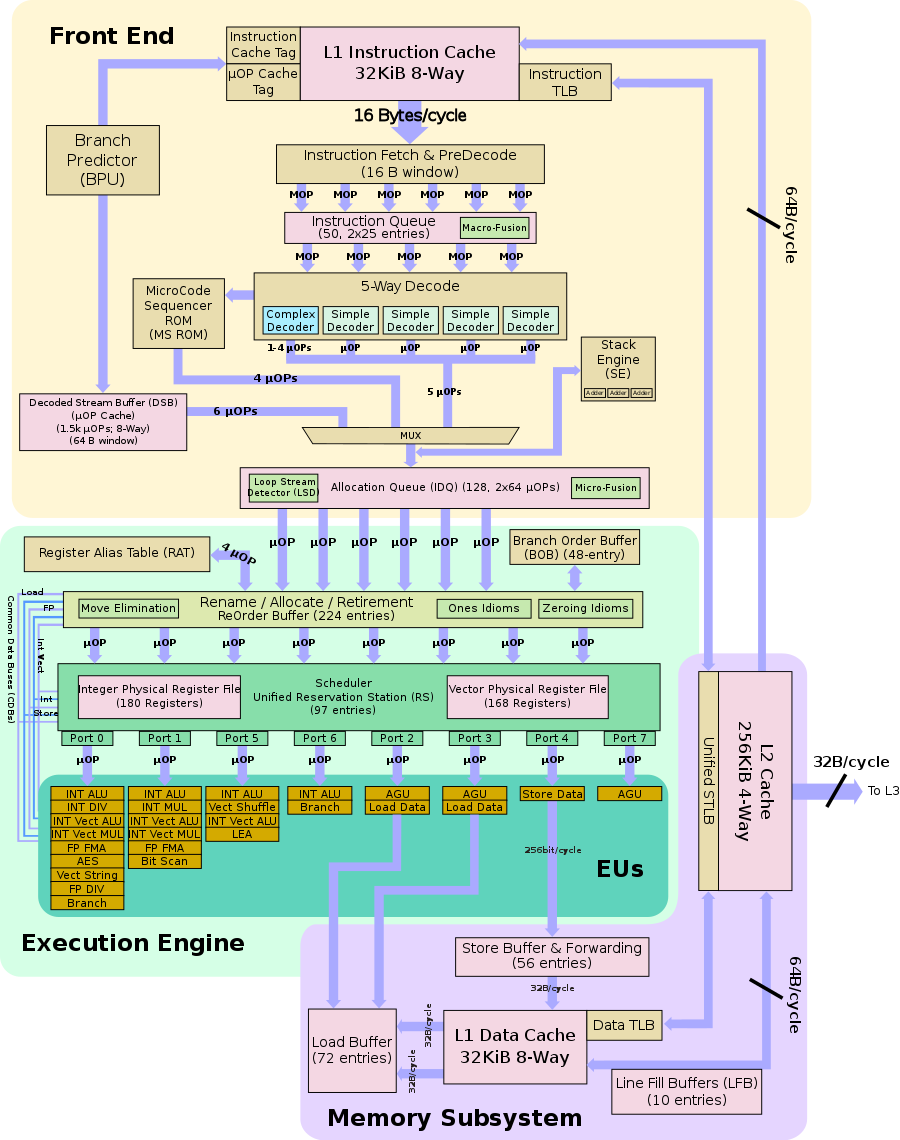
\includegraphics[width=0.94\textwidth]{./imgs/kaby.png}
      \end{center}
   \end{minipage}

   Για τον προσωπικό μου υπολογιστή, ο επεξεργαστής του Intel Core 
   \textbf{i7-8550U}
   χρησιμοποιεί την αρχιτεκτονική Kaby Lake.
   (https://en.wikichip.org/wiki/intel/microarchitectures/kaby\_lake).

   Όπως φαίνεται στο διάγραμμα, η αρχιτεκτονική Kaby Lake χρησιμοποιεί
   \textbf{ReOrder Buffer με 224 entries} (window size) και \textbf{Dispatch
   Width = 6 εντολές}. Σύμφωνα με την ανάλυση που προηγήθηκε, η επιλογή των
   χαρακτηριστικών αυτών είναι απολύτως λογική και δικαιολογητέα, αφού
   επιτυγχάνει αρκετά καλή απόδοση λαμβάνοντας υπ' όψιν το περιορισμένο μέγεθος
   chip και την χαμηλή κατανάλωση ενέργειας, εφόσον μάλιστα πρόκειται για
   επεξεργαστή προορισμένο για χρήση σε laptop. 


\end{document}